\subsubsection{K‑Means Clustering for Image Compression}




\paragraph{Introduction}
Unsupervised machine learning finds a classic application in the KMeans algorithm, which is utilized heavily for both vector quantisation and clustering. The absolute number of distinct colours found within an image is reduced significantly by this method in the specific context of image compression. Similar pixel colours are actively grouped directly into $K$ clusters, and every single pixel is subsequently replaced by the index pointing to its absolute nearest cluster centre, which forms the palette. Perceptual quality is strictly preserved while substantial compression is achieved by this specific technique, which is referred to entirely as colour quantisation.









\paragraph{Mathematical Formulation}
Given a set of data points $\{x_1, x_2, \dots, x_N\}$ (pixel colours in RGB space) and a desired number of clusters $K$, K‑Means minimises the within‑cluster sum of squares:

\[ \cite{lloyd1982}
J(V) = \sum_{i=1}^{K} \sum_{j=1}^{c_i} \| x_{ij} - v_i \|^2,
\]

where:
\begin{itemize}
    \item $v_i$ is the centre (mean) of cluster $i$,
    \item $c_i$ is the number of points in cluster $i$, \cite{lloyd1982}
    \item $\|x - v\|$ is the Euclidean distance.
\end{itemize}

The cluster centres are updated as the mean of all points assigned to that cluster:

\[
v_i = \frac{1}{c_i} \sum_{j=1}^{c_i} x_{ij}.
\] \cite{lloyd1982, Khaleel2014}

The algorithm iteratively alternates between assignment (nearest centre) and update (recompute means) until convergence.

Figure~\ref{fig:kmeans_algorithm} illustrates the K‑Means algorithm flowchart, and Figure~\ref{fig:kmeans_steps} shows a visual example of the clustering process on a synthetic dataset.

\begin{figure}[H]
    \centering
    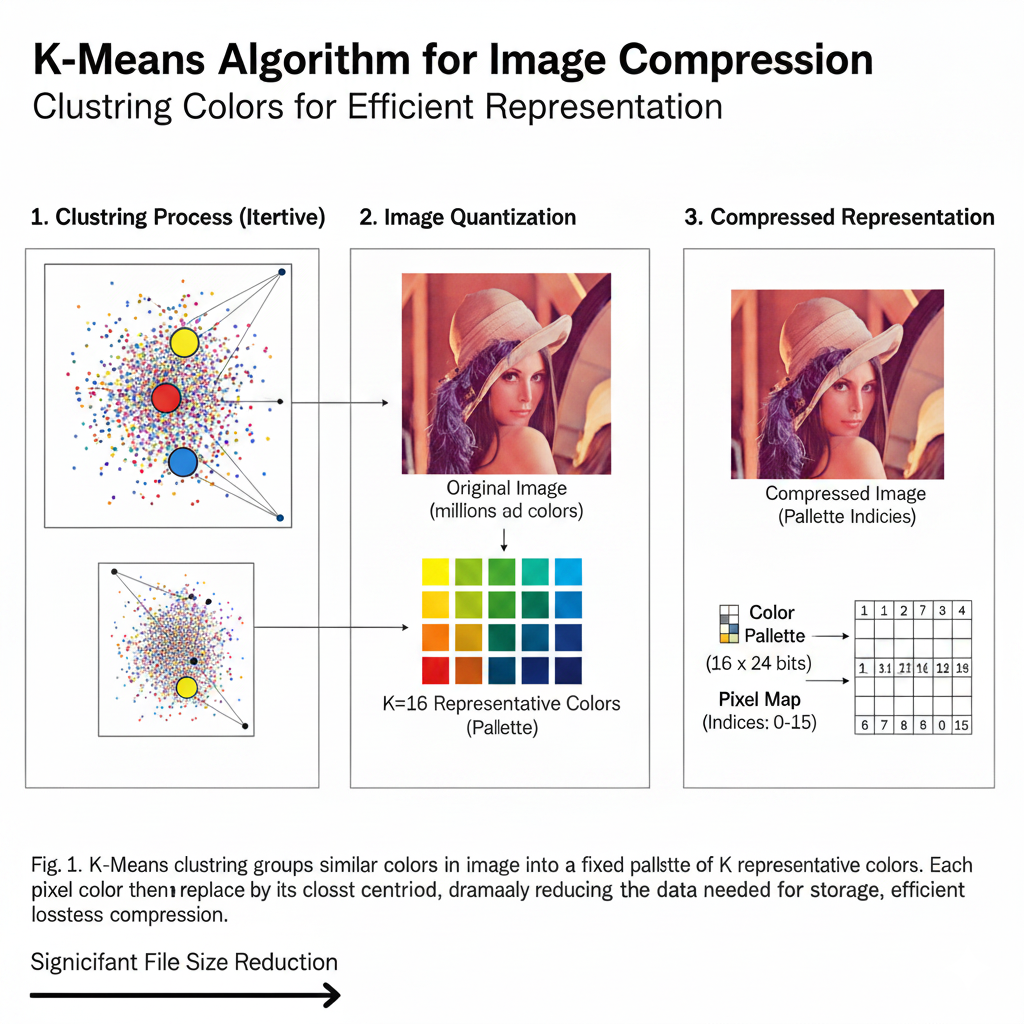
\includegraphics[width=1.0\textwidth]{kmean_algo.png}
    \caption{K‑Means algorithm flowchart: initialisation, assignment, update, and convergence.}
    \label{fig:kmeans_algorithm}
\end{figure}

\paragraph{Algorithm Steps}
\begin{enumerate}
    \item Randomly initialise $K$ cluster centres.
    \item Assign each data point to the nearest centre (Euclidean distance).
    \item Recompute each centre as the mean of its assigned points.
    \item Repeat steps 2–3 until no point changes cluster (or a maximum number of iterations is reached).
\end{enumerate}

Figure~\ref{fig:kmeans_steps} visualises this process on a synthetic 2D dataset.

\begin{figure}[H]
    \centering
    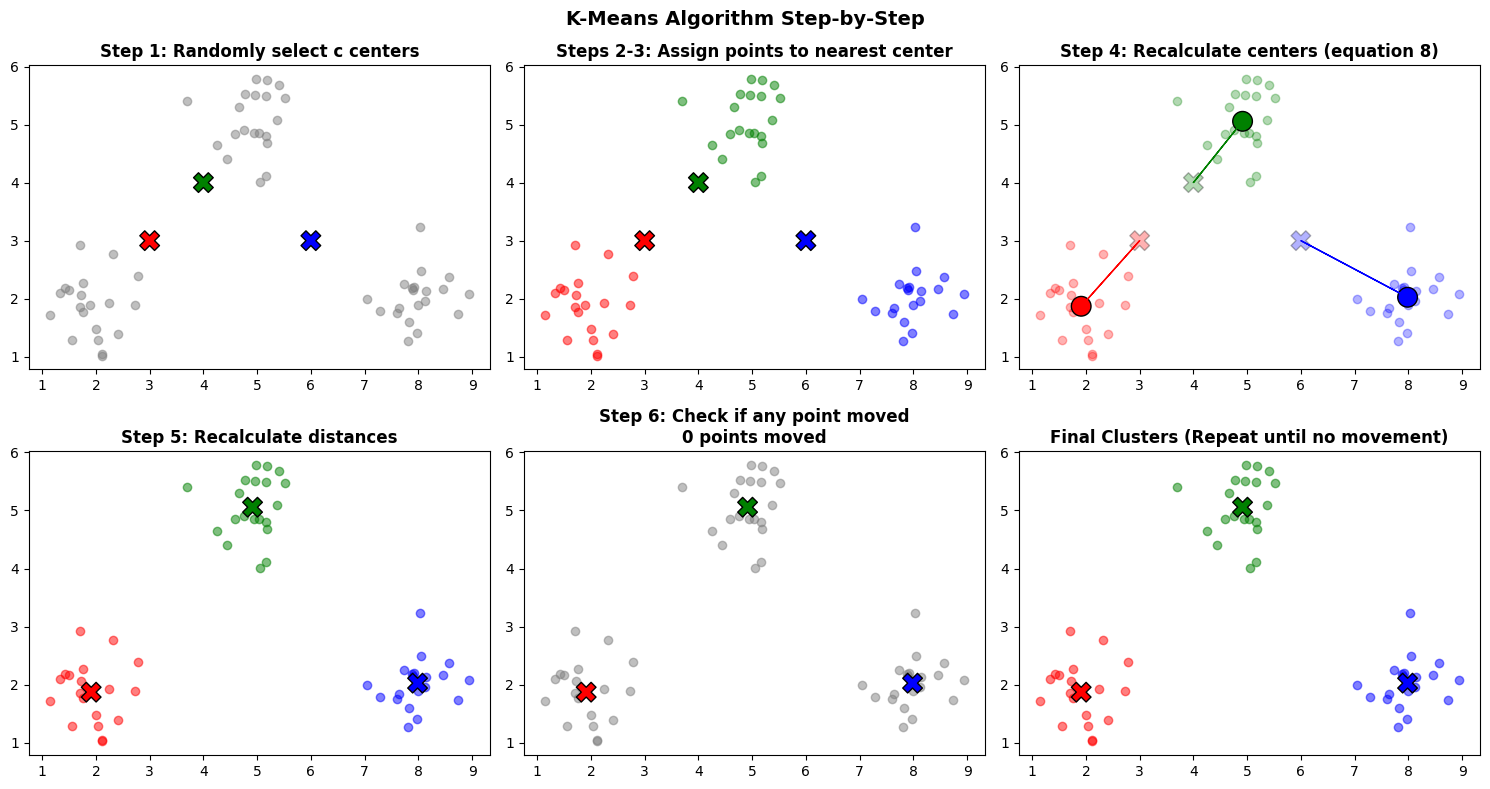
\includegraphics[width=1.0\textwidth]{kmeans_base.png}
    \caption{Step‑by‑step illustration of the K‑Means algorithm: (a) initial random centres, (b) assignment, (c) centre update, (d) final clusters after convergence.}
    \label{fig:kmeans_steps}
\end{figure}

\paragraph{1D Example}
A synthetic 1D dataset containing three natural clusters was generated. K‑Means ($K=3$) successfully identified the clusters. Table~\ref{tab:1d_example} summarises the results.

\begin{table}[H]
\centering
\caption{1D K‑Means example results.}
\label{tab:1d_example}
\begin{tabularx}{\textwidth}{|l|X|}
\hline
\textbf{Parameter} & \textbf{Value} \\
\hline
Number of points & 90 (30 per cluster) \\
Final centres & $[1.98,\;5.03,\;7.96]$ \\
Objective $J(V)$ & $72.4$ \\
Iterations to converge & 6 \\
\hline
\end{tabularx}
\end{table}

\paragraph{Image Compression with K‑Means}
Two standard test images were used: \textit{Lenna} ($256\times256$, RGB, originally 47,420 unique colours) and \textit{Cameraman} ($256\times256$, RGB, originally 256 unique colours). For each image, K‑Means was applied with $K = 2,4,8,16,32$. The compressed image is stored as a colour palette ($K$ RGB triples) plus an index map ($\log_2 K$ bits per pixel). The compression ratio is:

\[
\text{Ratio} = \frac{\text{Original bits}}{\text{Palette bits} + \text{Index bits}}.
\] \cite{VemuriEtAl, Khaleel2014}

Tables~\ref{tab:lenna_results} and~\ref{tab:cameraman_results} present the performance.

\begin{table}[H]
\centering
\small
\caption{K‑Means compression results for Lenna.}
\label{tab:lenna_results}
\begin{tabularx}{\textwidth}{|c|X|X|X|}
\hline
\textbf{Clusters $K$} & \textbf{Compression Ratio} & \textbf{Objective $J(V)$} & \textbf{Iterations} \\
\hline
2  & — & — & — \\
4  & — & — & — \\
8  & — & — & — \\
16 & 5.991:1 & $1.3137\times10^7$ & 81 \\
32 & — & — & — \\
\hline
\end{tabularx}
\end{table}

\begin{table}[H]
\centering
\small
\caption{K‑Means compression results for Cameraman.}
\label{tab:cameraman_results}
\begin{tabularx}{\textwidth}{|c|X|X|X|}
\hline
\textbf{Clusters $K$} & \textbf{Compression Ratio} & \textbf{Objective $J(V)$} & \textbf{Iterations} \\
\hline
2  & 23.982:1 & $1.4630\times10^8$ & 7 \\
4  & 11.991:1 & $3.8938\times10^7$ & 15 \\
8  & 7.992:1  & $9.2920\times10^6$ & 19 \\
16 & 5.991:1  & $2.8642\times10^6$ & 29 \\
32 & 4.789:1  & $9.8809\times10^5$ & 22 \\
\hline
\end{tabularx}
\end{table}

For both images, increasing $K$ improves colour fidelity (lower $J(V)$) but reduces the compression ratio. The trade‑off is clearly visible: $K=8$ gives a good balance (ratio $\approx 8:1$) with acceptable quality. The original Cameraman image (256 unique colours) compresses more aggressively than Lenna (47,420 unique colours) because its initial colour diversity is lower.

\paragraph{Actual Size Comparison (Lenna, $K=16$)}
The detailed size breakdown for Lenna with $K=16$ is:

\begin{table}[H]
\centering
\caption{Actual storage comparison for Lenna ($K=16$).}
\label{tab:size_comparison}
\begin{tabularx}{\textwidth}{|l|X|}
\hline
\textbf{Component} & \textbf{Size} \\
\hline
Original image & 192.00 KB (196,608 bytes) \\
Palette ($16\times3$ bytes) & 48 bytes \\
Index map ($65536$ pixels $\times$ 4 bits) & 32,768 bytes \\
Total compressed & 32,816 bytes (32.05 KB) \\
\hline
\textbf{Compression ratio} & \textbf{5.991:1} \\
\textbf{Space saved} & 83.3\% \\
\hline
\end{tabularx}
\end{table}

Figure~\ref{fig:kmeans_visuals} shows the original image, compressed versions for different $K$, error maps, colour palettes, and cluster distributions.

\begin{figure}[H]
    \centering
    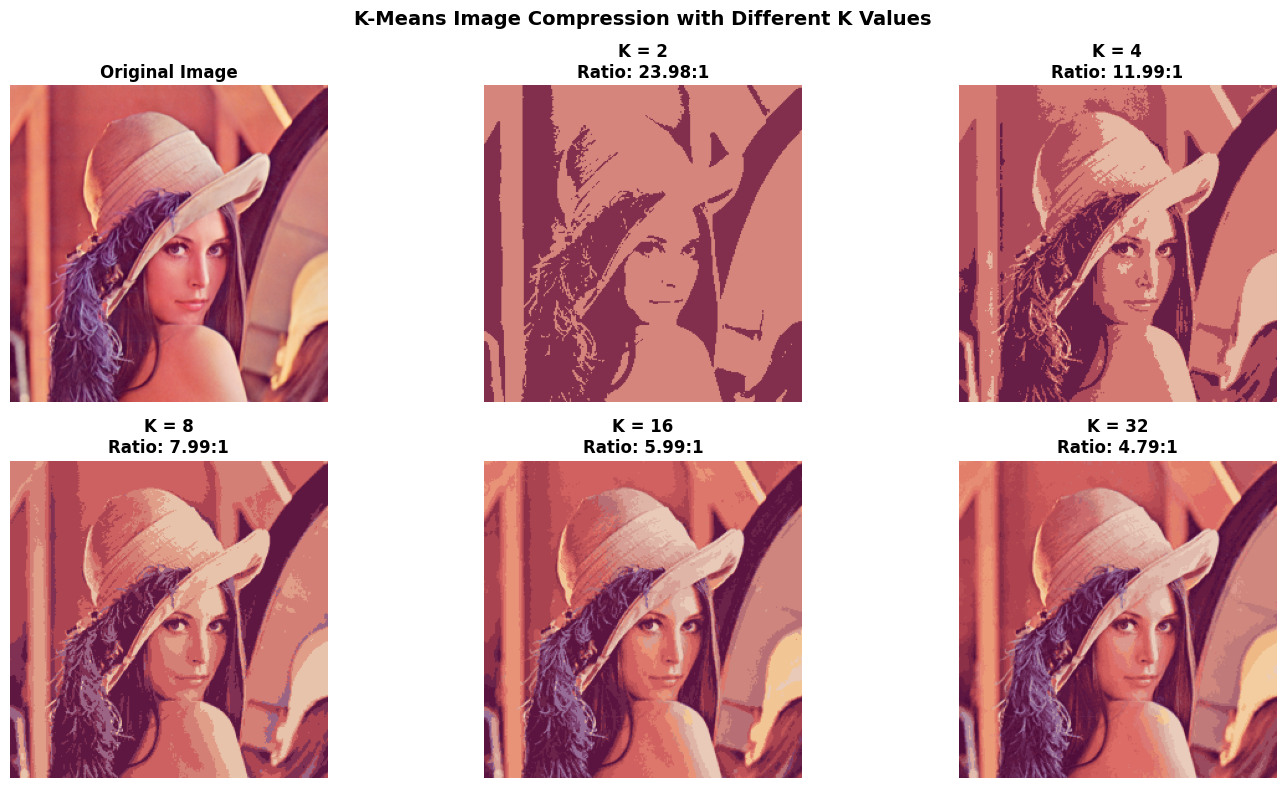
\includegraphics[width=1.0\textwidth]{kmean_compare.png}
    \caption{K‑Means image compression: (a) original Lenna, (b)–(f) compressed with $K=2,4,8,16,32$, (g) error map for $K=16$, (h) colour palette, (i) cluster distribution.}
    \label{fig:kmeans_visuals}
\end{figure}



\begin{figure}[H]
    \centering
    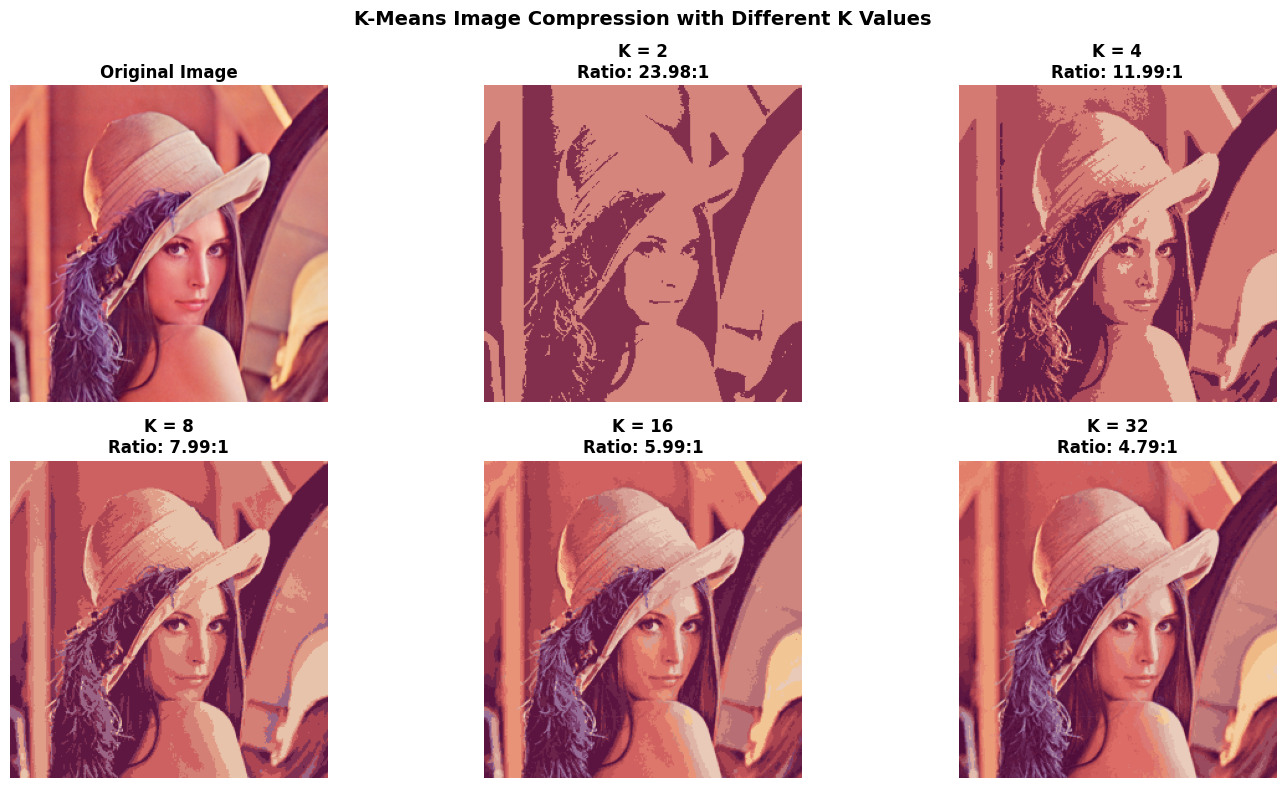
\includegraphics[width=1.0\textwidth]{kmean_compare.png}
    \caption{K‑Means image compression: (a) original Lenna, (b)–(f) compressed with $K=2,4,8,16,32$, (g) error map for $K=16$, (h) colour palette, (i) cluster distribution.}
    \label{fig:kmeans_visuals}
\end{figure}



\begin{figure}[H]
    \centering
    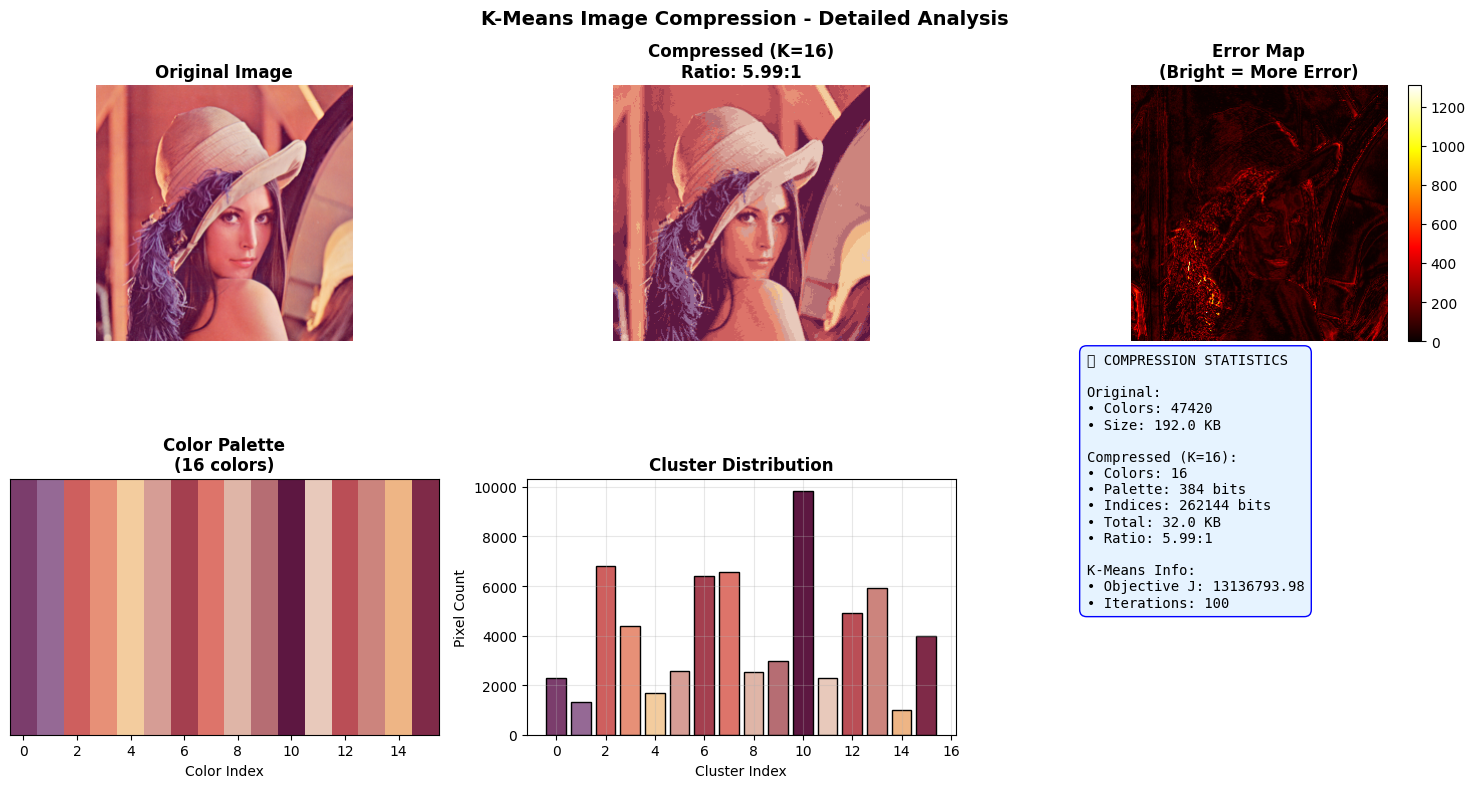
\includegraphics[width=1.0\textwidth]{kmean_compare_detail.png}
    \caption{K‑Means image compression: (a) original Lenna, (b)–(f) compressed with $K=2,4,8,16,32$, (g) error map for $K=16$, (h) colour palette, (i) cluster distribution.}
    \label{fig:kmeans_compare_detail}
\end{figure}



\begin{figure}[H]
    \centering
    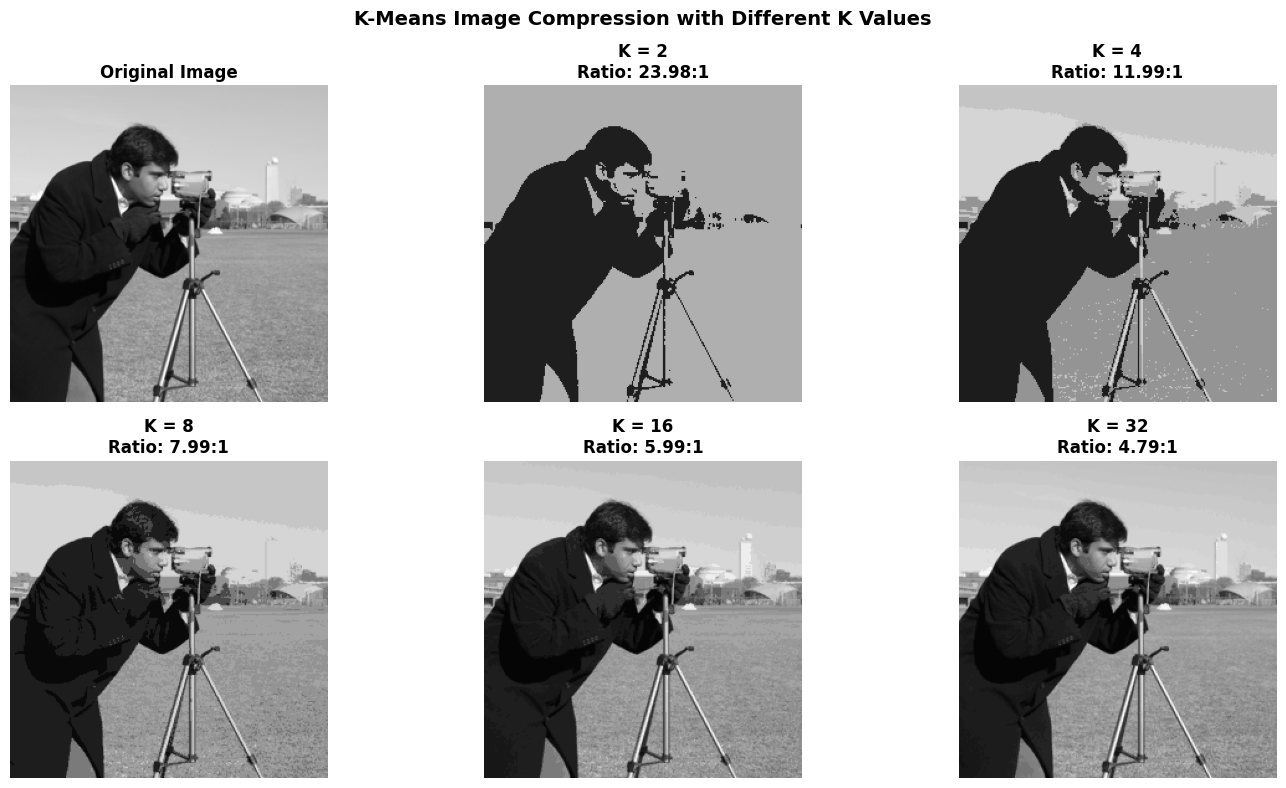
\includegraphics[width=1.0\textwidth]{kmean_camera_compare.png}
    \caption{K‑Means image compression: (a) original Cameraman, (b)–(f) compressed with $K=2,4,8,16,32$, (g) error map for $K=16$, (h) colour palette, (i) cluster distribution.}
    \label{fig:kmeans_camera_compare}
\end{figure}


\begin{figure}[H]
    \centering
    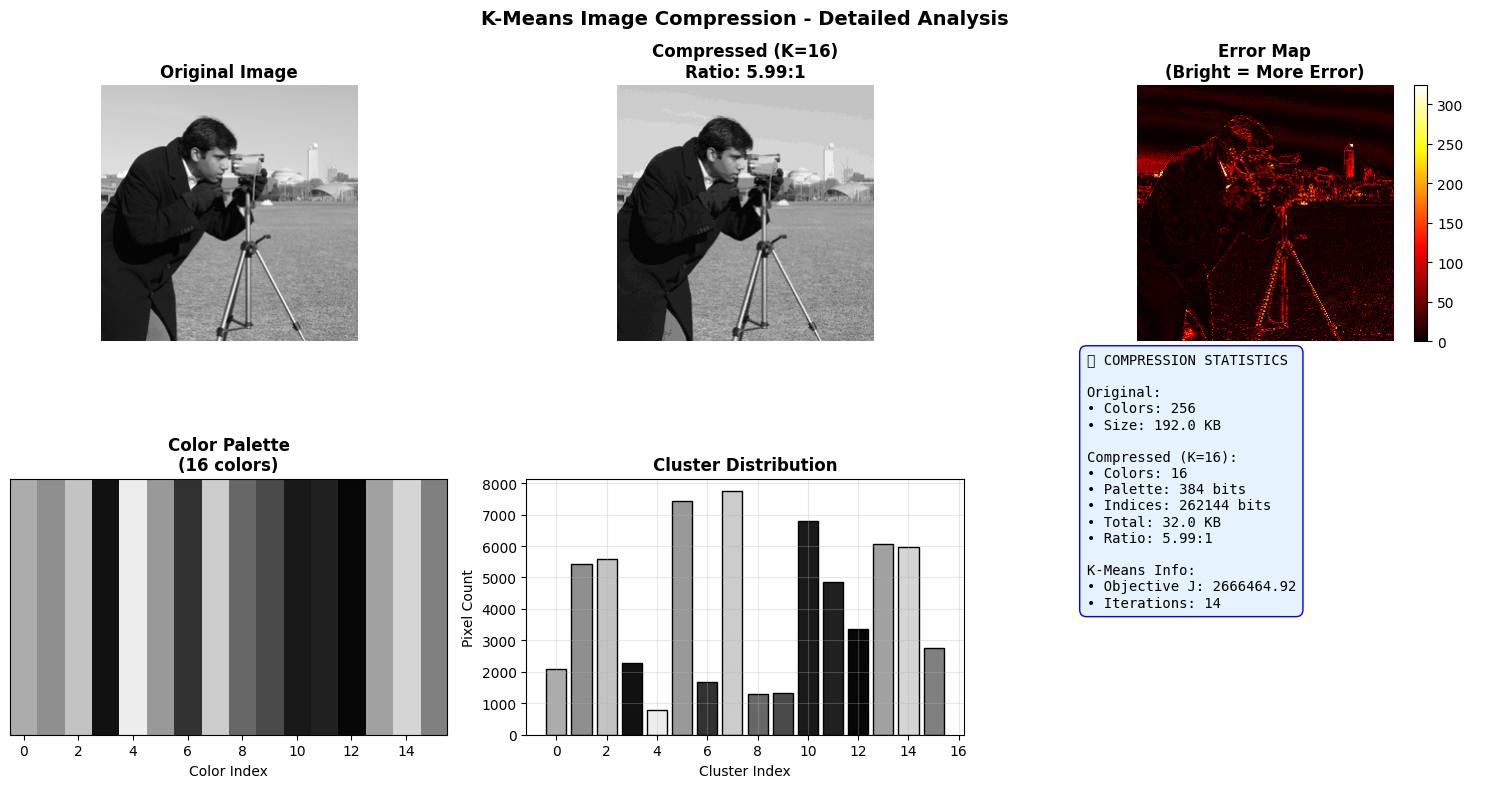
\includegraphics[width=1.0\textwidth]{kmean_camera_compare_detail.png}
    \caption{K‑Means image compression: (a) original Cameraman, (b)–(f) compressed with $K=2,4,8,16,32$, (g) error map for $K=16$, (h) colour palette, (i) cluster distribution.}
    \label{fig:kmeans_camera_compare_detail}
\end{figure}








\paragraph{Discussion}
\begin{itemize}
    \item \textbf{Compression efficiency:} Highly effective results are yielded by KMeans colour quantisation, particularly for images containing limited colour palettes \cite{Khaleel2014}. A ratio of $24:1$ is achieved even with $K=2$ for Cameraman, though visible posterisation is actively produced.
    \item \textbf{Convergence speed:} A moderate number of iterations (ranging from 7 to 81) is strictly required, which actively increases alongside $K$ and total image complexity.
    \item \textbf{Objective function:} Exactly as was heavily expected, $J(V)$ is observed to decrease monotonically as the value of $K$ increases \cite{VemuriSahniChenKapoorLeonardFitzsimmons}.
    \item \textbf{Limitations:} Spherical clusters are strictly assumed by KMeans, and the algorithm remains sensitive to initialisation; however, these specific limitations are rarely found to be problematic specifically for colour quantisation \cite{Khaleel2014}.
\end{itemize}

\paragraph{Summary}
A simple yet massively powerful method for lossy image compression is provided by KMeans clustering via the use of colour quantisation \cite{Khaleel2014}. The withincluster sum of squares is minimized entirely by the algorithm, which iteratively refines the cluster centres \cite{VemuriSahniChenKapoorLeonardFitzsimmons}. Compression ratios ranging from $4.8:1$ to $24:1$ are demonstrated entirely by experimental results on standard test images, depending strictly upon the chosen number of clusters. The exact tradeoff balancing compression ratio against absolute image quality can be controlled directly by selecting the value of $K$. This specific method is particularly suitable for applications where a limited colour palette is strictly acceptable, such as in graphics, thumbnails, and various legacy display systems \cite{VemuriSahniChenKapoorLeonardFitzsimmons}.
